\documentclass{standalone}
\usepackage{tikz}
\usepackage{amsmath} % for mathematical symbols

% TikZ settings
\tikzset{
    block/.style={draw, rectangle, minimum height=3em, minimum width=6em},
    line/.style={->, thick},
    every node/.append style={font=\footnotesize}
}

\begin{document}
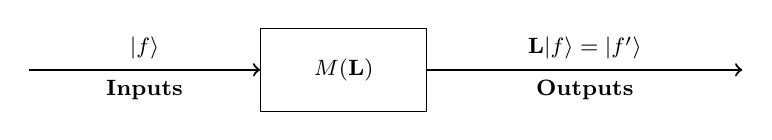
\begin{tikzpicture}[node distance=2cm]

    % Central block
    \node[block] (system) at (0,0) {$M(\mathbf{L})$};

    % Input line and label
    \draw[line] (-4,0) -- node[above] {$|f\rangle$} node[below] {\textbf{Inputs}} (system.west);

    % Output line and label
    \draw[line] (system.east) -- node[above] {$\mathbf{L}|f\rangle = |f'\rangle$} node[below] {\textbf{Outputs}} ++(4,0);

\end{tikzpicture}
\end{document}